\begin{figure}
	\centering
	\subcaptionbox{\label{fig:disoTPS_TEBD_global_update_TEBD1_splitting}}
	{%
		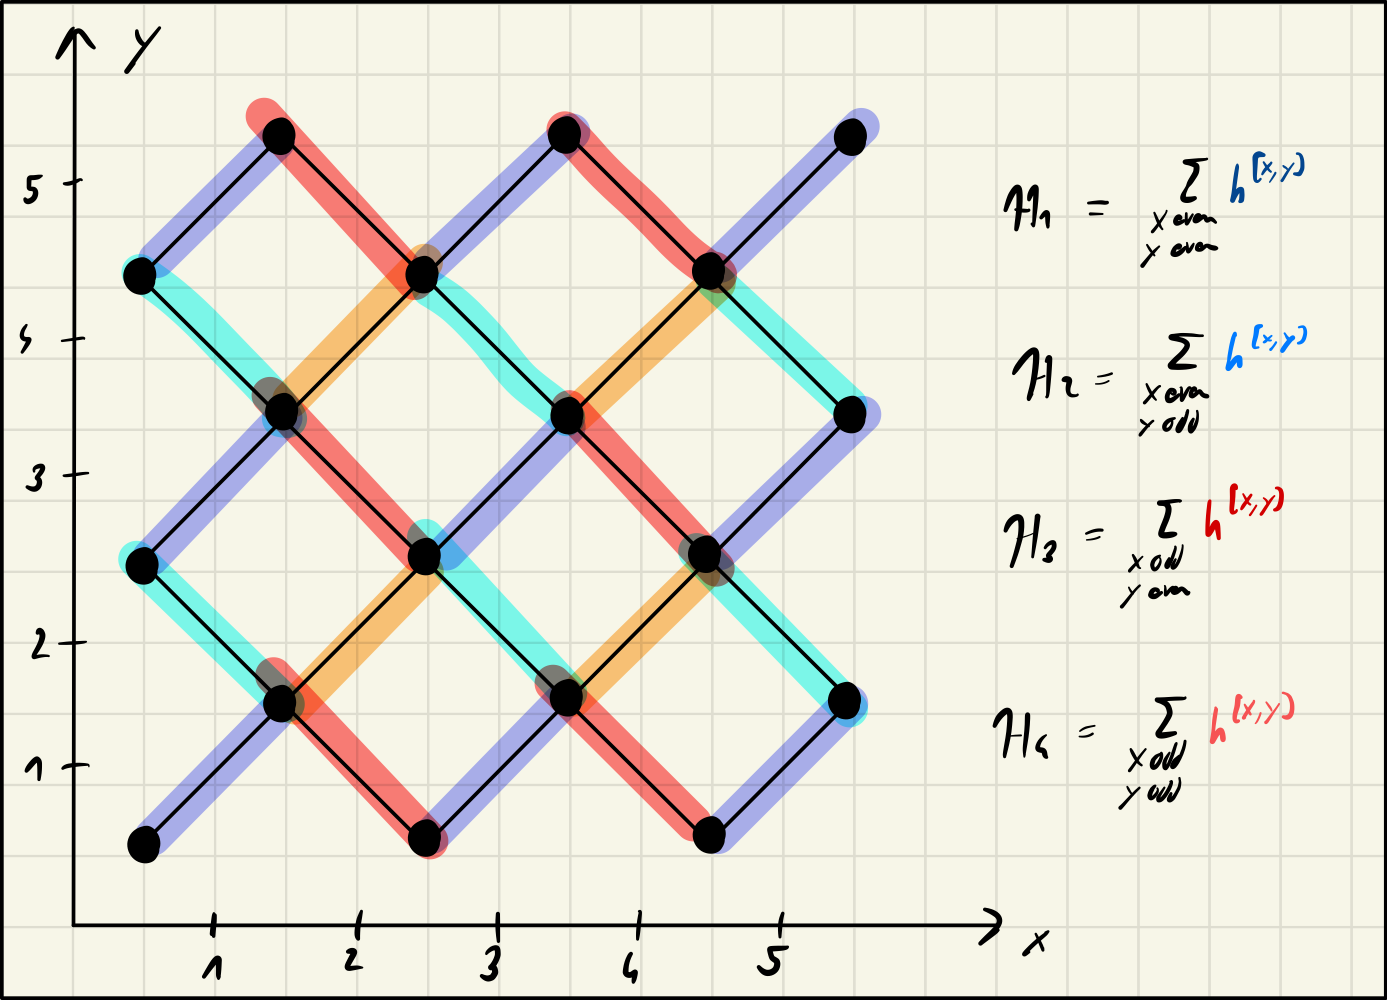
\includegraphics[width=0.6\textwidth]{figures/disoTPS/disoTPS_TEBD_global_update_TEBD1_splitting.jpeg}
	}
	\subcaptionbox{\label{fig:disoTPS_TEBD_global_update_TEBD2_chain}}
	{%
		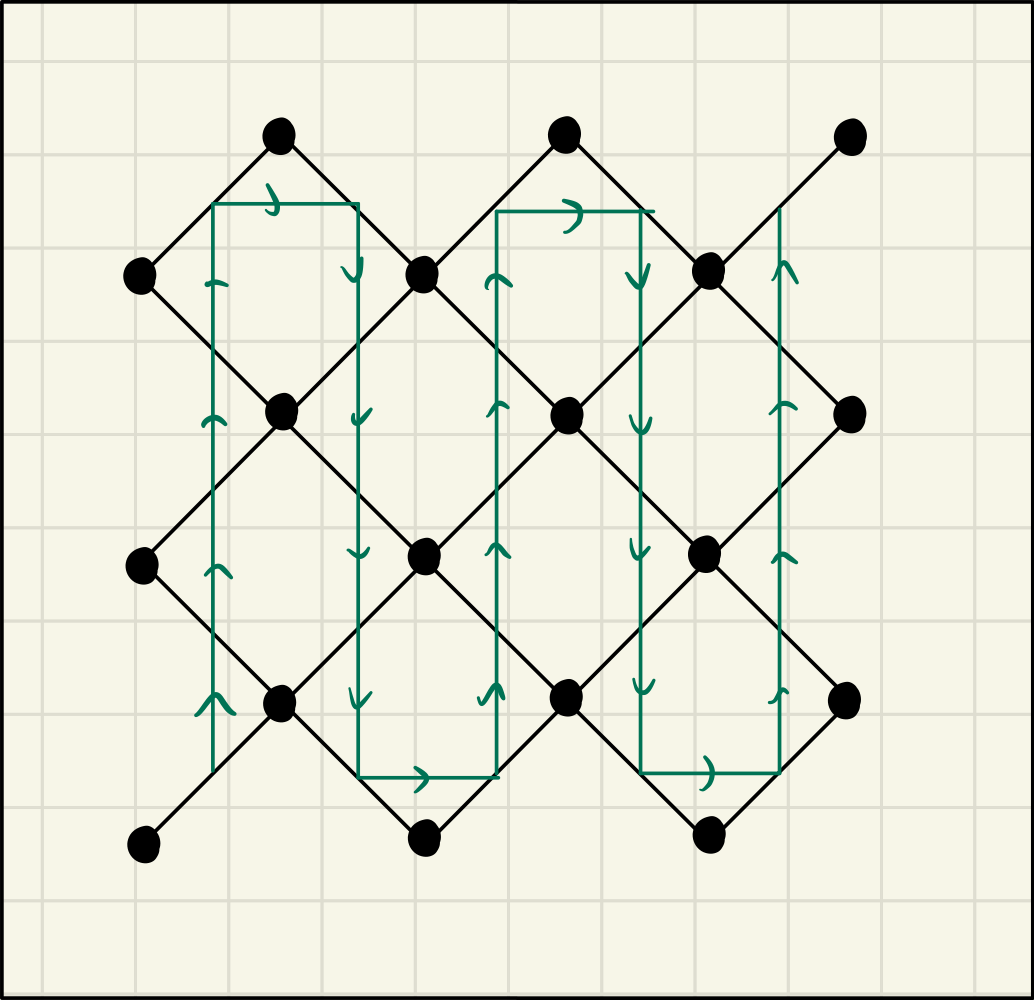
\includegraphics[width=0.6\textwidth]{figures/disoTPS/disoTPS_TEBD_global_update_TEBD2_chain.jpeg}
	}
	\caption{(a) A Hamiltonian $\hat{H}$ that is a sum of nearest-neighbour operators $h^{[x,y]}$ can be split into four parts made up of operators acting only on even/odd columns and even/odd bonds along a column. (b) A second order Suzuki-Trotter decomposition results in a chain of bond operators that have to be applied in the order visualized, moving along the path from the start to the end and backwards to the start again.}
	\label{fig:disoTPS_TEBD_global_update_TEBD1_splitting_and_TEBD2_chain}
\end{figure}
A global TEBD update evolves the state by a time $\Delta t$ and can be performed by applying local TEBD updates on all bonds. For each local TEBD update, the orthogonality center must be moved to the bond at which the update is applied. Because moving the orthogonality hypersurface can only be done approximately, the number of necessary moves should be minimized. \par
As we have already done for MPS in section \ref{sec:tensors_and_tensor_networks_matrix_product_states} let us assume that the Hamiltonian $\hat{H}$ can be written as a sum of nearest-neighbour operators. We index these nearest-neighbour operators $h^{[x, y]}$ by two integers $x$ and $y$ corresponding to the position of the orthogonality hypersurface and orthogonality center if moved to the bond on which $h^{[x,y]}$ acts. We define $x$ to increase from left to right and $y$ to increase from bottom to top, as shown in figure \figref{fig:disoTPS_TEBD_global_update_TEBD1_splitting}. The Hamiltonian can then be split into four parts by first grouping the $h^{[x,y]}$ into two sets acting only on even and odd columns respectively and then splitting each set again into terms acting only on even/odd bonds along the respective columns. We can write this as
\begin{equation}
	\label{eq:disoTPS_TEBD_splitting_local_Hamiltonian}
	\begin{split}
		\hat{H} = \sum_{x=1}^{2L_x-1} \sum_{y=1}^{2L_y-1}h^{[x,y]} &= \sum_{\substack{x\text{ even}\\y\text{ even}}} h^{[x, y]} + \sum_{\substack{x\text{ even}\\y\text{ odd}}} h^{[x, y]} + \sum_{\substack{x\text{ odd}\\y\text{ even}}} h^{[x, y]} + \sum_{\substack{x\text{ odd}\\y\text{ odd}}} h^{[x, y]} \\
		&\eqqcolon \hat{H}_1 + \hat{H}_2 + \hat{H}_3 + \hat{H}_4,
	\end{split}
\end{equation}
see also figure \figref{fig:disoTPS_TEBD_global_update_TEBD1_splitting}. The operators appearing in the sum in $\hat{H}_j$ commute with each other and thus the exponential $e^{-i\Delta t\hat{H}_j}$ factorizes into a product of bond operators $\hat{U}^{[x, y]}(\Delta t) = e^{-i\Delta t\hat{h}^{[x, y]}}$. \par
We next use a Suzuki-Trotter decomposition to approximate the time evolution operator
\begin{equation}
	\label{eq:disoTPS_TEBD_suzuki_trotter_first_order}
	\hat{U}(\Delta t) = \hat{U}^\text{TEBD1}(\Delta t) + \mathcal{O}(\Delta t^2)
\end{equation}
with
\begin{equation}
	\label{eq:disoTPS_TEBD_first_order_TEBD_operator}
	\hat{U}^\text{TEBD}(\Delta t) \coloneqq e^{-i\Delta t\hat{H}_4} e^{-i\Delta t\hat{H}_3} e^{-i\Delta t\hat{H}_2} e^{-i\Delta t\hat{H}_1}.
\end{equation}
To evolve the state $|\Psi\rangle$ in time with this first order approximation we must compute $|\Psi^\prime\rangle \approx U^\text{TEBD1}(\Delta t)|\Psi\rangle$ as a disoTPS. The procedure is sketched in figure \figref{fig:disoTPS_TEBD_global_update_applying_TEBD1}. We start in the left-most column and apply all bond operators that act on bonds along this column. The bond operators on the column are applied analogeously to the MPS algorithm: First we update all even bonds and then we update all odd bonds. Local updates are computed using the algorithm discussed in section \ref{sec:disoTPS_TEBD_local_updates}. Next, we move the orthogonality hypersurface two columns to the right and again apply all bond operators along the column. We proceed until all bond operators on even columns have been applied, in which case the orthogonality hypersurface is now positioned at its right-most position. We now sweep back to the left, applying all bond operators acting on odd columns along the way. Arriving back at the left-most column, all bonds making up $\hat{U}^\text{TEBD1}(\Delta t)$ have been applied in the correct order and the state has been evolved by time $\Delta t$. \par
\begin{figure}
	\centering
	\subcaptionbox{\label{fig:disoTPS_TEBD_global_update_applying_TEBD1}}
	{%
		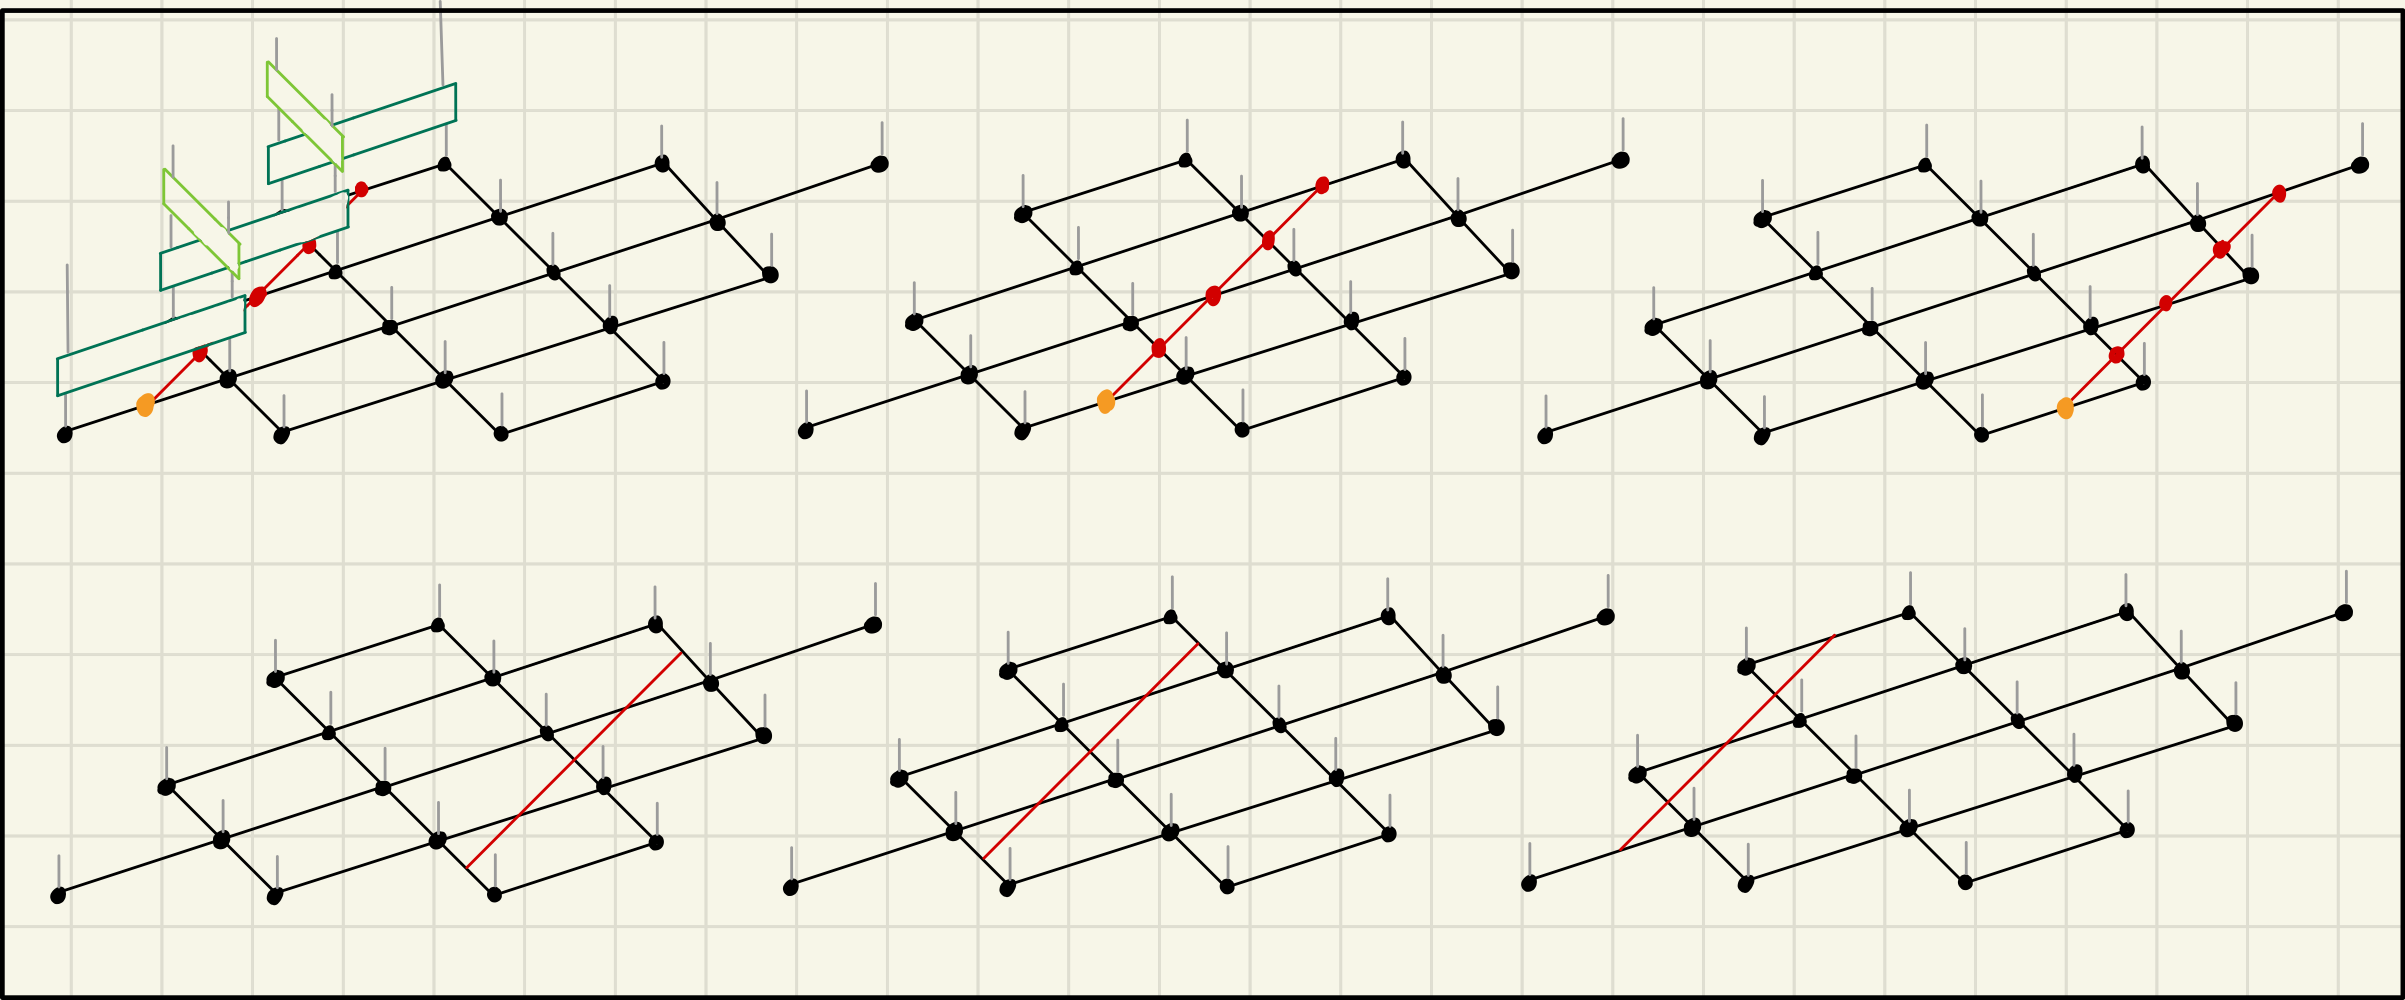
\includegraphics[width=1.0\textwidth]{figures/disoTPS/disoTPS_TEBD1_global_update.jpeg}
	}
	\subcaptionbox{\label{fig:disoTPS_TEBD_global_update_applying_TEBD2}}
	{%
		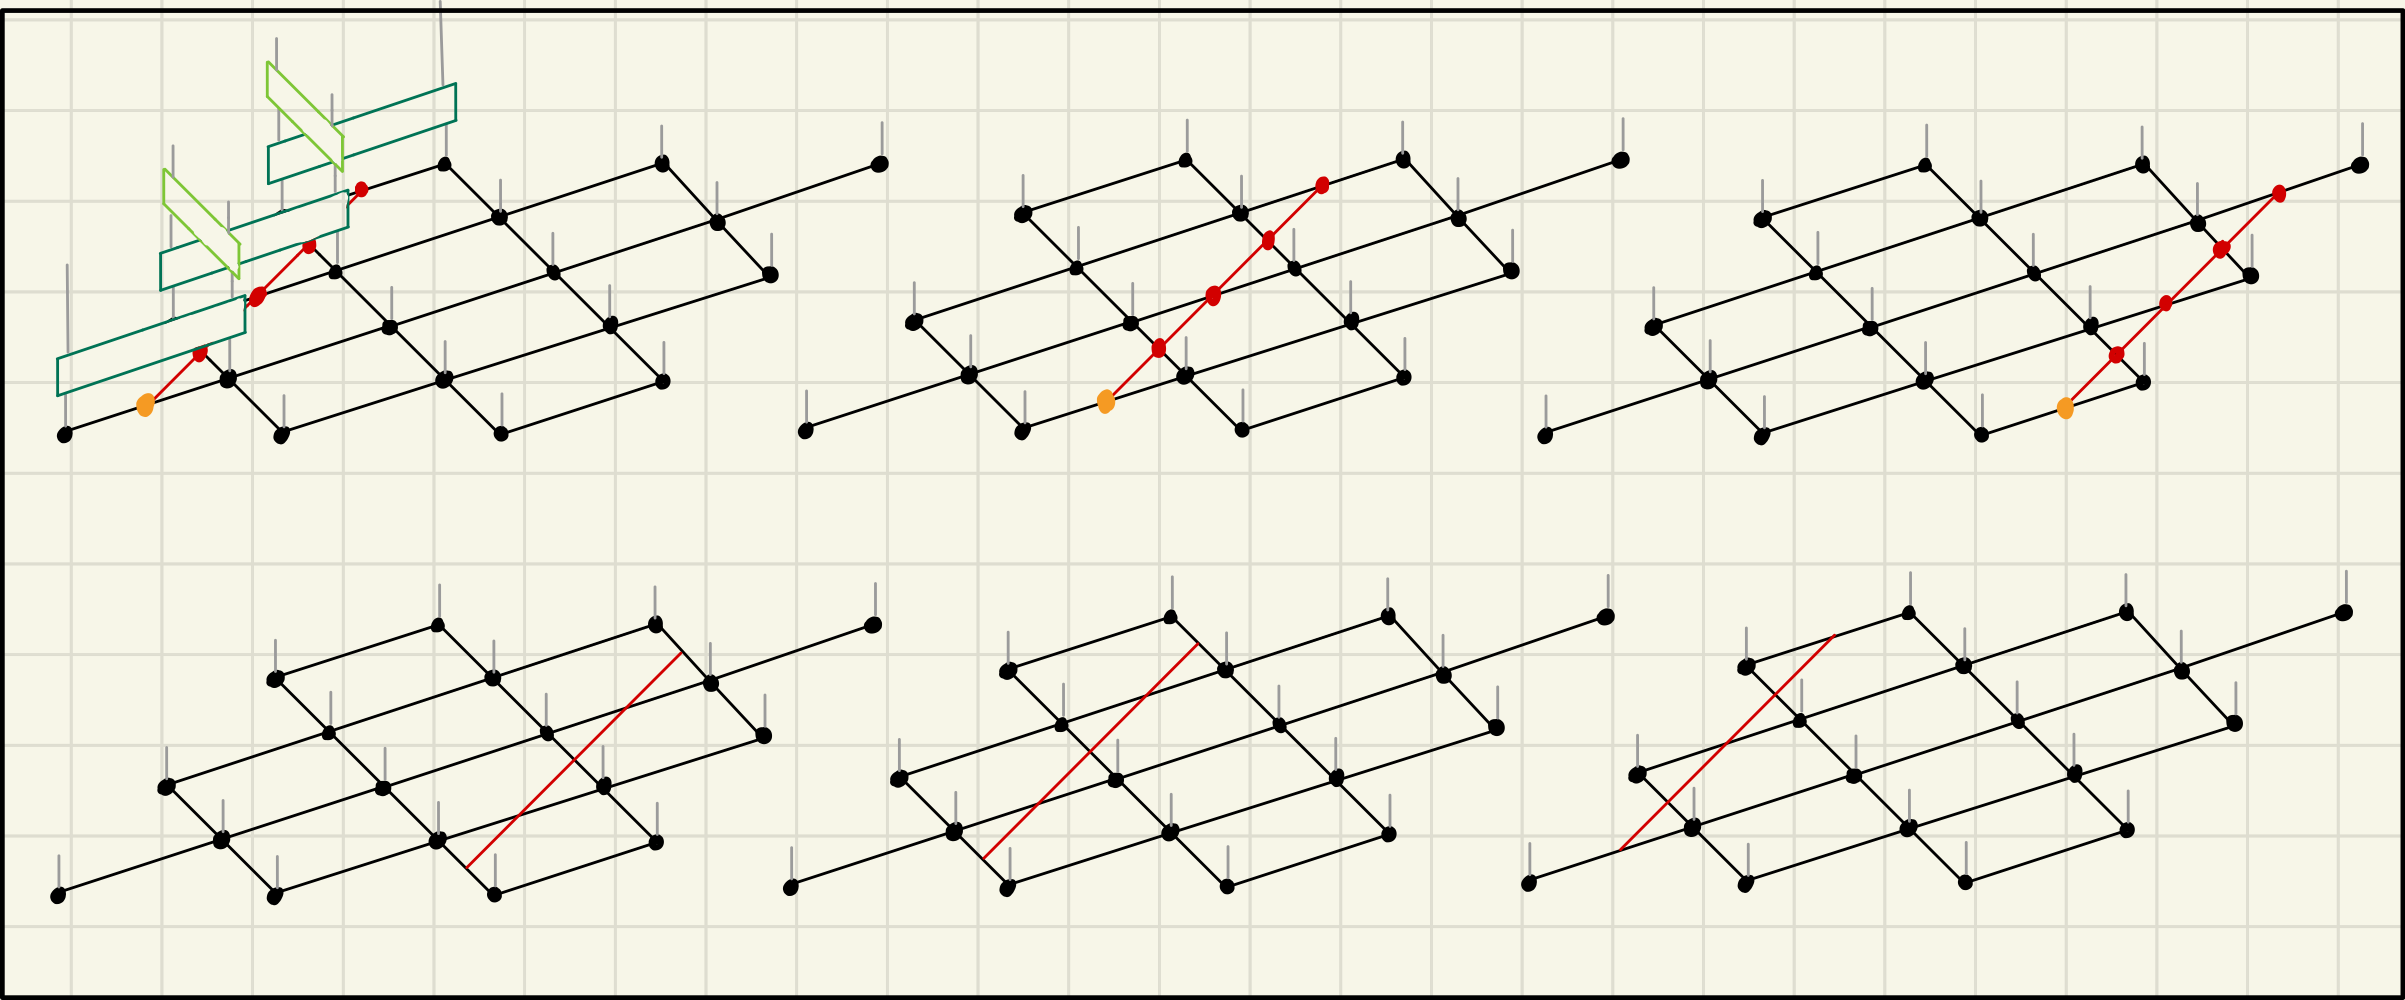
\includegraphics[width=1.0\textwidth]{figures/disoTPS/disoTPS_TEBD1_global_update.jpeg}
	}
	\caption{To apply a TEBD update of (b) first order and (b) second order, we sweep accross the disoTPS once from left to right and back from right to left. (a) TEBD1 applies the operators in a brick-wall fashion, while (b) TEBD2 applies the operators along a chain. \todo{The second picture should apply along a chain}}
	\label{fig:disoTPS_TEBD_global_update_applying_TEBD}
\end{figure}
We can obtain a better approximation of the time evolution operator $U(\Delta t)$ by performing a second order Suzuki-Trotter decomposition. By repeatedly applying the symmetrized decomposition
\begin{equation}
	e^{-i\varepsilon(A+B)} = e^{-i\frac{\varepsilon}{2}A}e^{-i\frac{\varepsilon}{2}A}e^{-i\varepsilon B} + \mathcal{O}(\Delta t^3)
\end{equation}
we obtain
\begin{equation}
	\begin{split}
		\label{eq:disoTPS_tebd_second_order_suzuki_trotter_decomposition}
		e^{-i\Delta t\hat{H}} &= \exp\left(-i\Delta t\sum_{x,y}\hat{h}^{[x,y]}\right) \\
		&= e^{-i\frac{\Delta t}{2}\hat{h}^{[1, 1]}} e^{-i\Delta t\left(\hat{H}-\hat{h}^{[1,1]}\right)} e^{-i\frac{\Delta t}{2}\hat{h}^{[1, 1]}} + \mathcal{O}(\Delta t^3)\\
		&= e^{-i\frac{\Delta t}{2}\hat{h}^{[1, 1]}} e^{-i\frac{\Delta t}{2}\hat{h}^{[1, 2]}} e^{-i\Delta t\left(\hat{H}-\hat{h}^{[1,1]}-\hat{h}^{[1, 2]}\right)} e^{-i\frac{\Delta t}{2}\hat{h}^{[1, 2]}} e^{-i\frac{\Delta t}{2}\hat{h}^{[1, 1]}} + \mathcal{O}(\Delta t^3)\\
		&=\cdots\\
		&= e^{-i\frac{\Delta t}{2}\hat{h}^{[1, 1]}} e^{-i\frac{\Delta t}{2}\hat{h}^{[1, 2]}} \cdots e^{-i\frac{\Delta t}{2}\hat{h}^{[1, 2]}} e^{-i\frac{\Delta t}{2}\hat{h}^{[1, 1]}} + \mathcal{O}(\Delta t^3).
	\end{split}
\end{equation}
Here, in each step we "split off" one operator $\hat{h}^{[x,y]}$ from the sum. The final result is a product of bond operators $\hat{U}^{[x,y]}(\Delta t/2))$ that must be applied from right to left. We can visualize this as a chain of bond operators that are applied along the path sketched in figure \figref{fig:disoTPS_TEBD_global_update_TEBD2_chain}. We start from the bottom left of the lattice, visiting every bond, and ending up on the top right. The same string of bond operators must then be applied backwards until arriving again at the bottom left. \par
The algorithm of applying a global update is thus similar to a TEBD update of first order. We sweep across the disoTPS once from left to right and back, applying bond operators along the way in the correct order, as visualized in figure \figref{fig:disoTPS_TEBD_global_update_applying_TEBD2}. The number of YB moves for TEBD1 and TEBD2 is the same, but the smaller Trotter error of $\mathcal{O}(\Delta t^3)$ instead of $\mathcal{O}(\Delta t^2)$ allows us to use larger time steps for TEBD2, resulting in a smaller number of YB moves per unit time. We find that the YB move is the primary source of error in practice and thus expect TEBD2 to perform much better than TEBD1. \par 
In principle, one could also go to higher decomposition orders \cite{cite:finding_exponential_product_formulas_of_higher_orders}. However, already a third order decomposition would necessitate a larger number of sweeps for applying the full update, increasing the error accumulated through YB moves. It is therefore not clear if higher order decompositions would be able to improve the method further.
